
\chapter{UNDERCONSTRUCTION. no proofreading at all!!!!!....   Experimental Results}
\label{chap:exp}

This chapter presents the experiments and the results when it comes to the evaluation of the following methods. A propose robot-camera calibration method and the 3D object pose estimation method. As to the robot-camera calibration method, the internal parameters of the camera to be calibrated need to be estimated. Methods for estimating the internal parameters also known as intrinsic parameters of the camera already exists and two of the most popular methods available in the open source community were selected. A detail description of those methods is in \ref{chap:robot}. In order to validate the output of the methods, a reprojection error as the standard metric is selected in this thesis. Then, with the most accurate internal parameters, the camera-robot calibration proceeds. A repeatability test, a validation test for the result of the robot-camera calibration follows. And finally, with the most accurate result of the robot-camera calibration, experiments for testing the 3D pose estimation system follows. For the purpose of testing, an industrial object is required as well as its CAD model. The latter is accomplished with the use of the FreeCAD software \ref{freecadb}, then, a suitable scaling undergoes with the use of CluodCompare software \ref{cloudcompareb}, where a point cloud is generated. As to the validation of the method, a ground truth of the object needs to be known in advance. For such a requirement. A checkboard is used as described in Figure \ref{setupsystem1} and Figure \ref{setupsystem2}. Then, by placing the robot TCP to the specific points (three points in totally), the checkerboard can be localized. With that, a new workspace is produced. By analyzing the translation and rotation errors, the system is evaluated.\\
The checkboard workspace is used for a rough estimation of the object's pose which is compared with 3D object pose estimation system described in \ref{chap:theo}.  


\section{Robot-Camera Calibration on the Yumi robot}
In order to get the best and accurate estimation of the robot-camera pose, careful attention must be given to the internal parameters of the camera which is a determinant factor of how accurate the extrinsic parameters are. For such estimation of those parameters, two methods were selected and the whole detail to both of them is shown in \ref{chap:robot}. The Astra camera and the RealSense camera are used in this thesis.  The cameras are calibrated with the methods previously mention and their results are shown in \ref{-------------------}. As to the validation process, a reprojection error is used. Since it is one of the most used metrics,  it is used in this thesis. 

\subsection{Reprojection Error}

The reprojection error is the distance between a pattern keypoint detected in a calibration image, and a corresponding world point projected into the same image. Figure \ref{fig:realopen} and Figure \ref{fig:realros} show the calibration results by analyzing the reprojection error per image when the camera is a RealSense with the OpenCV and camera \textunderscore industrial calibration methods. As to, Figure \ref{fig:astraopen} and Figure \ref{fig:astraros} show the calibration results when the case is with an Astra camera, with the same procedure, by analyzing the reprojection error per image with both methods, the OpenCV and camera \textunderscore industrial calibration.



%%%%%%%%%%%%%%%%%%%%%%%%%%%%%%%%%%%%%%%%%%
\begin{figure}[!h]
\begin{center}
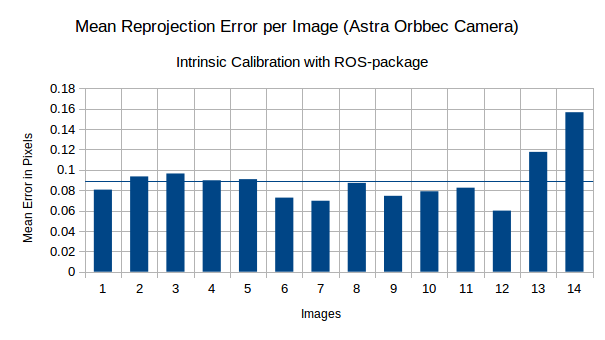
\includegraphics[width=5in, height=3.5in]{figures05/ros_int_cal_astra.png}
\caption{Mean Reprojection Error per image with a ROS method (Astra Orbbec Camera)}%\cite{temp2}}
\label{fig:astraros}
\end{center}
\end{figure}

\begin{figure}[!h]
\begin{center}
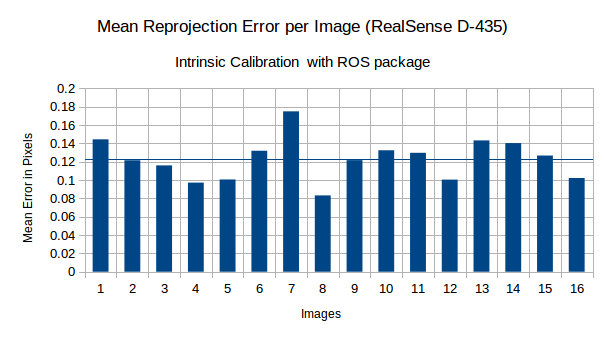
\includegraphics[width=5in, height=3.5in]{figures05/ros_int_cal_real.png}
\caption{Mean Reprojection Error per image with a ROS method (RealSense D-435)}%\cite{temp2}}
\label{fig:realros}
\end{center}
\end{figure}

\begin{figure}[!h]
\begin{center}
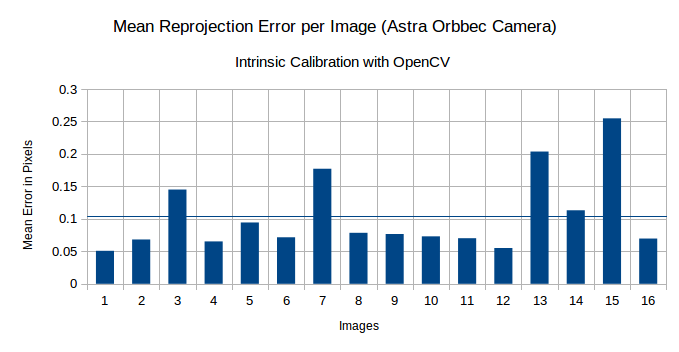
\includegraphics[width=5in, height=3.5in]{figures05/opencv_int_cal_astra.png}
\caption{Mean Reprojection Error per image with a OpenCV method (Astra Orbbec Camera)}%\cite{temp2}}
\label{fig:astraopen}
\end{center}
\end{figure}

\begin{figure}[!h]
\begin{center}
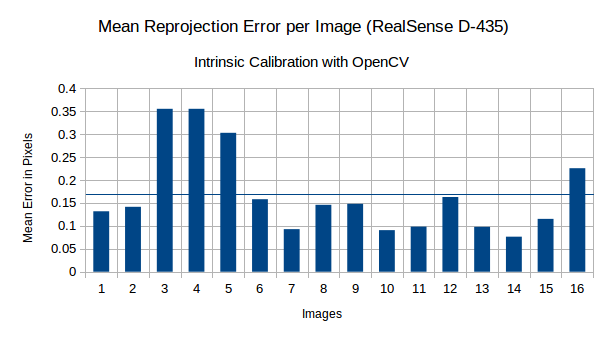
\includegraphics[width=5in, height=3.5in]{figures05/opencv_int_cal_real.png}
\caption{Mean Reprojection Error per image with a OpenCV method (RealSense D-435)}%\cite{temp2}}
\label{fig:realopen}
\end{center}
\end{figure}

In order to discuss the result for each case, an average error is calculated for each case. This is done by computing the arithmetical mean of the errors calculated for all the calibration images. And that result should be as close to zero as possible according to the literature in computer vision.

\subsection{Result Analysis}
After computing the average error for both cameras, the results are shown in Table \ref{astra1} related to the Astra camera and Table \ref{real1} which corresponds to the RealSense D-435.\\
 It can be seen that the overall mean error representing the Astra camera is quite correlated to one another. by that we meant, the reprojection error obtained from OpenCV and camera \textunderscore industrial calibration is very similar with a small offset. But that difference is acceptable due to it holds the requirement to be under the 0.5 pixels, a specified value in the literature for determining how accurate a device sensor is. \\
On the other hand, the results for the RealSense camera are not quite correlated. Several thoughts can be drawn from that result. The sensor might be quite sensitive to changes in the calibration target resulting in taking wrong measurements. In addition to that, the light condition can also affect the sensory device since the data taken is an RGB image. Such difference presented in the mean reprojection error can hugely affect the good accurate the output of the estimation of the camera frame relative to the robot frame by applying the eye-to-hand calibration. In order to confirm that this different holds. We proceeded to take new measurements, with the careful attention of not moving the calibration target when the sensory device is taken its sample. Then the whole process is evaluated again. The difference holds between methods, but meet the requirements of being under the 0,5 pixels. With the result in hand is quite early to conclude that the RealSense camera is or is not a good choice for solving the main problem of this master Part localization for robotic manipulation. By keeping that difference in mind, we proceed with the next experiment for validating the robot-camera calibration.  \\
As a remark, both cameras were calibrated with same light conditions, with the same calibration target and with an equal number of images. Considering, all in all, it can be concluded that the Astra camera seems to perform well and it can be our final choice for the pose estimation system evaluation. 

\begin{table}[ht]
\renewcommand{\arraystretch}{1.3}
\caption{Experiment data for internal Astra sensor calibration.}
\label{astra1}
\centering
\begin{tabular}{|c||c|}
\hline
Method & Overall Mean Error\\
\hline
OpenCV &  0.1041954808\\
\hline
ROS &  0.1081118023\\
\hline
\hline
\end{tabular}
\end{table}

\begin{table}[ht]
\renewcommand{\arraystretch}{1.3}
\caption{Experiment data for internal RealSense sensor calibration.}
\label{real1}
\centering
\begin{tabular}{|c||c|}
\hline
Method & Overall Mean Error\\
\hline
OpenCV &  0.1684388411\\
\hline
ROS &  0.122868849\\
\hline
\hline
\end{tabular}
\end{table}

\subsection{Eye-To-Hand Calibration}

The second experiment in this chapter is related to the eye-to-hand calibration. In this experiment, both cameras, the Astra and RealSense again, are taken into account for the validation test. Since the quality of the extrinsic calibration depends on how good the estimation of the internal parameters is, we proceed with taking the best accurate internal parameters based on the reprojection error as described previously, where the less reprojection error the camera has, the more accurate the camera is. \\
By defining the best internal parameters, the validation test to run is divided into two types. In the first type of experiment also called a validation test. The calibration plate with a checkerboard place on it as described in \ref{chap: robot} is kept at a constant angle, parallel to the XY plane of the robot coordinate system. Figure \ref{setupext} shows the basic setup for the extrinsic calibration with a constant orientation parallel to the XY plane of the robot during the whole process that takes it. The whole process includes movements with a small offset between every pose of the TCP (Tool Center Point). Where the joint configuration values for each pose is known in advance. The joint values were saved after each and suitable movement with the help of the handheld of the robot. Each one of those saved movement guarantees that the checkerboard is detected by the robot. Basically, the robot executes a translation of the TCP around the XY plane of itself.\\ 
As to the second experiment, where the calibration plate is tilting with predefined orientations. The same approach is taken, several joint values configuration is saved, provided that the checkboard is always detected by the camera to be calibrated. After defining the type of movement, several criteria for obtaining a reasonable estimation of the camera relative to the robot frame are taking into account. One of the consideration is related to the pause in between the movements, is set. This is with the aim to cancel the effects of possible vibrations that the robot can produce so that wrong measurement is avoided during the whole process of the extrinsic calibration. Another consideration is related to speed. A reasonable speed of $25\%$ is set for the validation test. \\

With the types of experiments knowing in advance, and main criteria to consider for each one of them. The execution of the robot movement follows. To be able to control the robot arm, interface one of both camera at each test, and estimate the pose of the camera relative to the robot base, three nodes were developed as described in \ref{chap:robot}. The node named as $publishingTF.py$ is responsible for controlling the robot move and publishing the transformation from the robot frame to TCP (Tool Center Point) frame into the ROS network (tf topic to be specific). \\
The second node named as $target\textunderscore locator \textunderscore astra.py$ or $target\textunderscore locator \textunderscore rsense.py$  which depends on the camera used, is responsible  for computing the estimation of the camera pose relative to the calibration target (checkerboard) frame. In addition to that, it broadcast that estimation of camera pose into the ROS network. A third node named $listeningTF.py$ is responsible for keeping track of the all coordinate frames over time, and querying for the transformation of the camera frame relative to the robot frame, as well as the computation of the average of the transformation it queries after each executed robot move. 

\subsection{Calibration results}

%%%%%%%%%%%%%%%%%%%%%%%%%%%%%%%%%% astra 
\begin{itemize}
\item The following eye-to-hand transform was obtained for the Astra Camera with the calibration plate parallel to the XY plane in robot frame:
\begin{equation}
^{R}T_{C}=\begin{bmatrix} -2.26051005e-02 & 7.30112611e-01 & -6.82952842e-01 & 1.19260379\\9.99481127e-01 & 8.25583772e-04 & -3.21992981e-02 & 0.12098781\\ -2.29452788e-02 & -6.83326345e-01 & -7.29752438e-01 & 0.53569317 \end{bmatrix}
\end{equation}

\item The following eye-to-hand transform was obtained for the Astra Camera by tilting the calibration plate:
\begin{equation}
^{R}T_{C}=\begin{bmatrix} -0.01440125 & 0.72431469 & -0.68931911 & 1.19518608\\0.99970886 & -0.00291747 & -0.02395149 & 0.11374275\\ -0.01935949 & -0.68946336 & -0.7240618 & 0.53606583 \end{bmatrix}
\end{equation}

%%%%%%%%%%%%%%%%%%%%%%%%%%%%%%%%% realsense

\item The following eye-to-hand transform was obtained for the RealSense D-435 camera with the calibration plate parallel to the XY plane in robot frame:
\begin{equation}
^{R}T_{C}=\begin{bmatrix} -2.23312402e-02 & 2.94145863e-01 & -9.55499622e-01 &1.22253213\\9.99723971e-01 & -4.09078692e-04 & -2.34907523e-02 & 0.11776472 \\ -7.30058216e-03 & -9.55760453e-01 & -2.94055535e-01 & 0.32424239  \end{bmatrix}
\end{equation}

\item The following eye-to-hand transform was obtained for the RealSense D-435 camera by tilting the calibration plate:
\begin{equation}
^{R}T_{C}=\begin{bmatrix} -0.01833338  0.30085851 -0.95349255 & 1.21972025\\0.99978158 -0.00405373 -0.02050249& 0.09386797\\ -0.01003355 -0.95366017 -0.30071848& 0.33192816\end{bmatrix}
\end{equation}
\end{itemize}

\subsection{Result Analysis}

The propose robot-camera calibration method was successfully performed provided that the calibration target was detected by the 3D camera to be calibrated. In order to validate whether the proposed method is accurate enough for the pose estimation system described in \ref{chap:robot} or not, ground truth is necessary to know in advance. But it was a challenging task to measure an exact orientation and translation of the camera with respect to the robot frame. Given that the housing of the camera (namely the RealSense camera) is rounded which makes it hard to get a good measurement from the mounting point to the camera. In addition to that, the orientation and the translation from the sensor to the housing is not known. It was proved that such difficulty is normal to encounter since the cameras used in this thesis are not suitable for the problem to be solved in this master thesis. Suitable cameras to work with, for the assignment of this thesis are the so-called industrial cameras where the camera frame is given. But that camera was not available.  
For the given conditions, a validation test is still considered. A rough estimation of the camera pose relative to the robot is measured. The measuring tape was used for the rough estimation but it is not considered as ground truth to evaluate the result of the robot-camera calibration but rather a good idea of what the result should be. \\
The repeatability test is proposed for the validation of the extrinsic parameters. It consists of repeating over again the whole process when it comes to the estimation of the external values, those who represent the camera pose relative to the robot frame. But a major difference is taking into account for this new test. The difference is that the new joint values are taken and saved provided that the checkerboard is detected by the camera used in turn and the number of movements is increased.\\
Given the previous condition, the repeatability test is executed. The results are shown in \ref{chap:resultsa}. Standard deviation and mean values are computed from those results. The mean values and standard deviation for the Astra camera are shown in Table \ref{meanastra1} and Table \ref{standardastra1} when the orientation of the camera is kept constant. When it comes to the type of experiments where the robot moves with tilting motion, the results are shown in Table \ref{meanastra2} and \ref{standardastra2}.\\
From the values, it can be seen that the external parameters differ from one to another in the range of 1cm for the x-axis and y-axis. As to the z-axis, 1mm is reported. Given that condition, it can be concluded that the external parameters for the Astra camera either with a fast test with few movements or thorough test which means more movements are acceptable.
As to the RealSense Camera, where the standard deviation and mean values are shown in Table \ref{meanreal1} and \ref{standardreal1} when a constant angle was the case. As to the case where a tilting angle is applied, the results are shown in Table \ref{meanreal2} and \ref{standardreal2}.\\
From the values, it can be seen that the external parameters differ approximately 1cm for the x-axis, 2cm for the y-axis and 1cm  when it comes to vertical displacement.  It can be concluded that the Astra is performed constant values in the repeatability test, compare to the RealSense camera. But a new validation test should be applied. 
By doing intrinsic calibration and the eye-to-hand calibration, the next and final validation test takes place for the 3D pose estimation system.

%%%%%%%%%%%%%%%%%%%%%%%%%%%%%%%For Astra Camera
\begin{table}[ht]
\renewcommand{\arraystretch}{1.3}
\caption{Mean Values of The Repeatability Test With a Constant Orientation of the Calibration Plate(Astra Camera).}
\label{meanastra1}
\centering
\begin{tabular}{|c||c||c||c||c||c||c|}
\hline
$x[m]$ & $y[m]$ & $z[m]$ & $q_{x}$ & $q_{y}$ & $q_{z}$ &$q_{\omega}$ \\
\hline
1.1926 & 0.1245 & 0.5368& 0.653175&	0.661978&	-0.269761&	-0.249755 \\
\hline
\hline
\end{tabular}
\end{table}
\begin{table}[ht]
\renewcommand{\arraystretch}{1.3}
\caption{Standard Deviation from The Repeatability Test With a Constant Orientation of the Calibration Plate(Astra Camera).}
\label{standardastra1}
\centering
\begin{tabular}{|c||c||c||c||c||c||c|}
\hline
$\sigma_{x[m]}$ & $\sigma_{y[m]}$ & $\sigma_{z[m]}$ & $\sigma_{q_{x}}$ & $\sigma_{q_{y}}$ & $\sigma_{q_{z}}$ &$\sigma_{q_{\omega}}$ \\
\hline
0.011012&	0.009877	&0.000906&0.000243&	8.45E-05&	0.000446&	0.000976\\
\hline
\hline
\end{tabular}
\end{table}
\begin{table}[ht]
\renewcommand{\arraystretch}{1.3}
\caption{Mean Values of The Repeatability Test With Tilting Motion of the Calibration Plate(Astra Camera).}
\label{meanastra2}
\centering
\begin{tabular}{|c||c||c||c||c||c||c|}
\hline
$x[m]$ & $y[m]$ & $z[m]$ & $q_{x}$ & $q_{y}$ & $q_{z}$ &$q_{\omega}$ \\
\hline
1.197089&	0.116571&	0.539509&
0.653488&	0.660281&	-0.270449&	-0.252499 \\
\hline
\hline
\end{tabular}
\end{table}
\begin{table}[ht]
\renewcommand{\arraystretch}{1.3}
\caption{Standard Deviation from The Repeatability Test With Tilting Orientation of the Calibration Plate(Astra Camera).}
\label{standardastra2}
\centering
\begin{tabular}{|c||c||c||c||c||c||c|}
\hline
$\sigma_{x[m]}$ & $\sigma_{y[m]}$ & $\sigma_{z[m]}$ & $\sigma_{q_{x}}$ & $\sigma_{q_{y}}$ & $\sigma_{q_{z}}$ &$\sigma_{q_{\omega}}$ \\
0.012046&	0.010473&	0.008465& 0.000837&	0.002155&	0.000920&	0.002450
\\
\hline
\hline
\end{tabular}
\end{table}
%%%%%%%%%%%%%%%%%%%%%%%%%%%%%%%%%%%%%%For Real Sense Camera
\begin{table}[ht]
\renewcommand{\arraystretch}{1.3}
\caption{Mean Values of The Repeatability Test With a Constant Orientation of the Calibration Plate(RealSense Camera).}
\label{meanreal1}
\centering
\begin{tabular}{|c||c||c||c||c||c||c|}
\hline
$x[m]$ & $y[m]$ & $z[m]$ & $q_{x}$ & $q_{y}$ & $q_{z}$ &$q_{\omega}$ \\
\hline
1.222425&	0.112532&	0.324441&0.564006&	0.573552&	-0.426780&	-0.413272 \\
\hline
\hline
\end{tabular}
\end{table}
\begin{table}[ht]
\renewcommand{\arraystretch}{1.3}
\caption{Standard Deviation from The Repeatability Test With a Constant Orientation of the Calibration Plate(RealSense).}
\label{standardreal1}
\centering
\begin{tabular}{|c||c||c||c||c||c||c|}
\hline
$\sigma_{x[m]}$ & $\sigma_{y[m]}$ & $\sigma_{z[m]}$ & $\sigma_{q_{x}}$ & $\sigma_{q_{y}}$ & $\sigma_{q_{z}}$ &$\sigma_{q_{\omega}}$ \\
\hline
0.000160&	0.007729&	0.000294&9.20E-05&	4.19E-05&	5.26E-05&	1.31E-05\\
\hline
\hline
\end{tabular}
\end{table}
\begin{table}[ht]
\renewcommand{\arraystretch}{1.3}
\caption{Mean Values of The Repeatability Test With Tilting Motion of the Calibration Plate(Real Sense).}
\label{meanreal2}
\centering
\begin{tabular}{|c||c||c||c||c||c||c|}
\hline
$x[m]$ & $y[m]$ & $z[m]$ & $q_{x}$ & $q_{y}$ & $q_{z}$ &$q_{\omega}$ \\
\hline
1.222425&	0.112532&	0.324441&0.564006&	0.573552&	-0.426780&	-0.413272  \\
\hline
\hline
\end{tabular}
\end{table}
\begin{table}[ht]
\renewcommand{\arraystretch}{1.3}
\caption{Standard Deviation from The Repeatability Test With Tilting Orientation of the Calibration Plate(RealSense Camera).}
\label{standardreal2}
\centering
\begin{tabular}{|c||c||c||c||c||c||c|}
\hline
$\sigma_{x[m]}$ & $\sigma_{y[m]}$ & $\sigma_{z[m]}$ & $\sigma_{q_{x}}$ & $\sigma_{q_{y}}$ & $\sigma_{q_{z}}$ &$\sigma_{q_{\omega}}$ \\
0.000160&	0.007729&	0.000294&9.20E-05&	4.19E-05&	5.26E-05&	1.31E-05\\
\hline
\hline
\end{tabular}
\end{table}

\section{Pose Estimation Pipeline}

This section presents the experiments and the results and how the validation test was performed for the 3D object pose estimation system. But first of all, for executing such an experiment, few requirements need to be met. The first requirement, a 3D industrial object, namely a textured object is available. As the second requirement, its CAD model is also available since it was created by the author of this thesis with the use of the FreeCAD software \ref{freecadb}. And last but not least, a third requirement, which is related to the pose of the object to be known in advance. This pose should be computed in a different fashion so that the result can be compared with the output of the pose estimation pipeline.\\
With the output from the pose estimation pipeline and the available pose which it is referred to as ground truth, the accuracy of the system can be determined. But, it was proved to be difficult to determine the real pose of the object for the given thesis research. But a solution needed to comes out for the ground truth refers to as a gold standard pose also in this thesis. Therefore, several methods were discussed knowing that the meaning of ground truth refers to as an information provided by direct observation such as an empirical observation. A simple and unusual solution is taking into account to  the ground truth. The use of the checkerboard pattern. Having the checkboard pattern place on the table, a localization object feature from the robot is used. This is done by position the TCP onto three different points of the checkerboard, by doing so, a new coordinates system is defined where the object is placed to a desired grid of the checkboard which width and hight is 2cm each. With such setup the object can be move as the author of this thesis wishes with a certain confident of know the deisplacement in XY coordinates of the plane of chessboard. As to the orientation, a digital angle ruler is used in this thesis. The whole setup for the experiment can be seen in Figure \ref{setupsystem2} where the checkerboard object is localized onto the top of the table. Figure \ref{setupsystem1} shows a rviz simulation, where the relationship between transformations are clearly seen over time. 

\subsection{Validation Test}\label{valitest}

In this section two type of experiments is taken place. The ultimate goal is to validate the pose estimation pipeline in terms of robustness and accuracy by the means of a distance error and an angle error. The pose estimation pipeline is described in \ref{chap:theo}, where it said that two 3D datas are required. One of them, a point cloud generated from the CAD model, and the other one, a point cloud generated from the scene, which was adquired from the output of the sensory device used, Astra or RealSense camera. The point cloud generated from the CAD model is called source cloud and the point cloud generated from the depth image is called the target cloud in this thesis.\\
In order to validate the first experiment, displacements and angles applied to the industrial object are executed. As to displacement, there are three types related to it, one in the x-axis, the other one in the y-axis and the last one in the XY plane of the chekerboard. The distance of such a displacement is 2cm each. Since the transformation of the checkboard is known in advance plus the displacement applied to the object, the rough object pose can be known by visul inspection of the author of this thesis. When it comes to the validation test for the angle, a digital angle ruler is used, and the orientation is applied on the z-axis, namely a clockwise rotation. For the validation of the second experiment, the same principle is applied as described above when it comes to change the pose of the objec around the XY plane of the checkerboard. But a major difference exists for the source point cloud (CAD model). The CAD model is substitute for a partially view point cloud generated the camera used. The change was applied in order to see whether exist or not an improvement. Since the pose estimation system from time to time failed for the given conditions in the first experiment.

\subsection{Pose Estimation Results}
 
For the case when when the source cloud is generated from CAD model and the target cloud from the sensory device as described in \ref{valitest}. The following Figure \ref{fig:errorx_1nd}, \ref{fig:errory_1nd}, and \ref{fig:erroryaw_1nd} where obtained for such experiment. It can bee seen that the estimated pose deviates slightly from its ground values.
%%%%%%%%%%%%%%%%%%%%%%%%%%% cloud from CAD and astra
\begin{figure}[!h]
\begin{center}
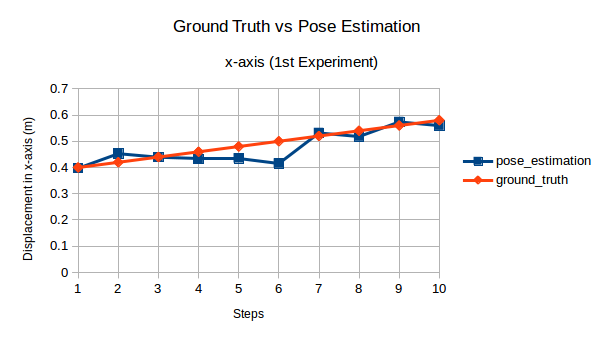
\includegraphics[width=5in, height=3.5in]{figures05/1_x_validation.png}
\caption{Ground Truth vs Pose Estimation: x-axis (1st Experiment)}
\label{fig:errorx_1nd}
\end{center}
\end{figure}
\begin{figure}[!h]
\begin{center}
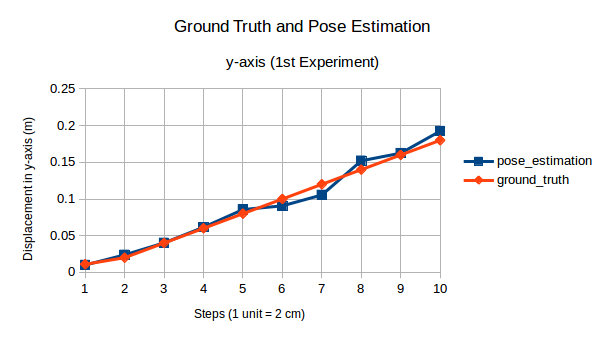
\includegraphics[width=5in, height=3.5in]{figures05/1_y_validation.png}
\caption{Ground Truth vs Pose Estimation: y-axis (1st Experiment)}
\label{fig:errory_1nd}
\end{center}
\end{figure}
\begin{figure}[!h]
\begin{center}
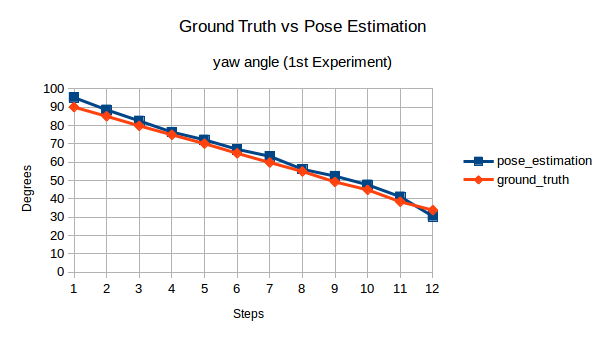
\includegraphics[width=5in, height=3.5in]{figures05/1_yaw_validation.png}
\caption{Ground Truth vs Pose Estimation: yaw angle (1st Experiment)}
\label{fig:erroryaw_1nd}
\end{center}
\end{figure}

For the case when when the source cloud as well as the target cloud are generated from the sensory device as described in \ref{valitest}. The Figure \ref{fig:errorx_2nd}, \ref{fig:errory_2nd}, and \ref{fig:erroryaw_2nd} where obtained for such experiment. It can bee seen that the estimated pose deviates slightly from its ground values.
%%%%%%%%%%%%%%%%%%%%%%%%%%%%% cloud from the same source
\begin{figure}[!h]
\begin{center}
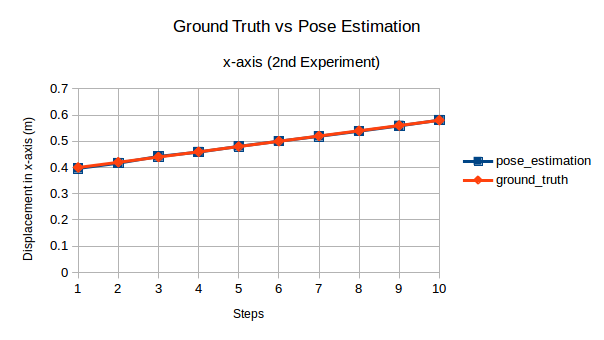
\includegraphics[width=5in, height=3.5in]{figures05/2_x_validation.png}
\caption{Ground Truth vs Pose Estimation: x-axis (2nd Experiment)}
\label{fig:errorx_2nd}
\end{center}
\end{figure}
\begin{figure}[!h]
\begin{center}
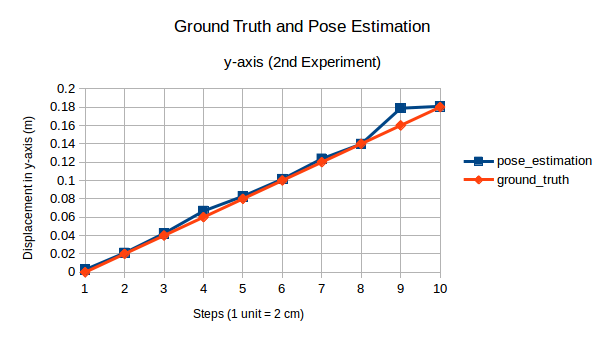
\includegraphics[width=5in, height=3.5in]{figures05/2_y_validation.png}
\caption{Ground Truth vs Pose Estimation: y-axis (2nd Experiment)}
\label{fig:errory_2nd}
\end{center}
\end{figure}
\begin{figure}[!h]
\begin{center}
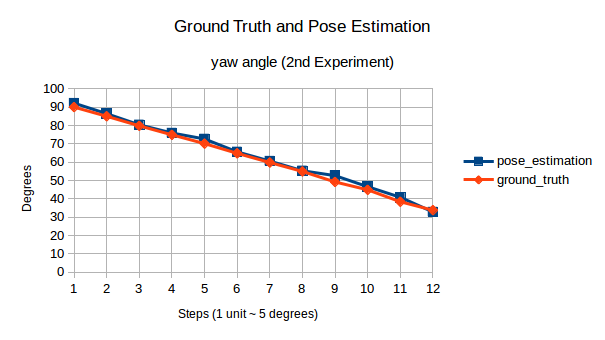
\includegraphics[width=5in, height=3.5in]{figures05/2_yaw_validation.png}
\caption{Ground Truth vs Pose Estimation: yaw angle (2nd Experiment)}
\label{fig:erroryaw_2nd}
\end{center}
\end{figure}

%%%%%%%%%%%%%%%%%%%%%%%%%%%
From the deviation graph an absolute error can be calculated. Figure \ref{fig:absx}, \ref{fig:absy} and \ref{fig:absw} show the error calculated for both experiments.

\begin{figure}[!h]
\begin{center}
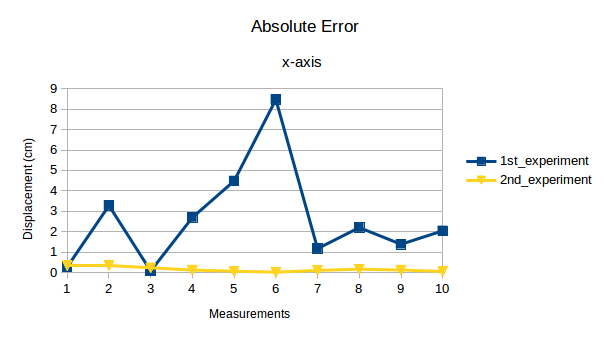
\includegraphics[width=5in, height=3.5in]{figures05/abs_error_x.png}
\caption{Absolute Error: x-axis}
\label{fig:absx}
\end{center}
\end{figure}

\begin{figure}[!h]
\begin{center}
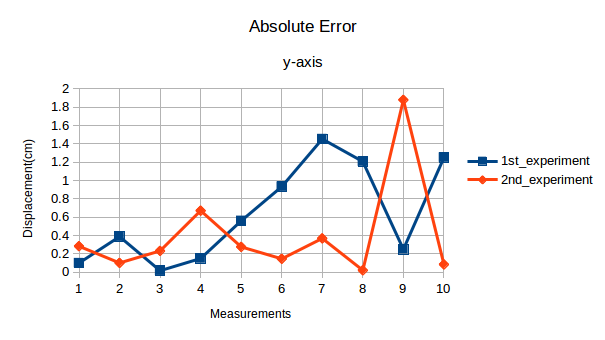
\includegraphics[width=5in, height=3.5in]{figures05/abs_error_y.png}
\caption{Absolute Error: y-axis}
\label{fig:absy}
\end{center}
\end{figure}

\begin{figure}[!h]
\begin{center}
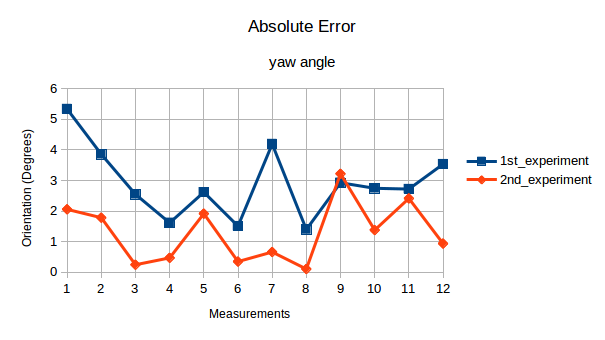
\includegraphics[width=5in, height=3.5in]{figures05/abs_error_yaw.png}
\caption{Absolute Error: yaw angle}
\label{fig:absw}
\end{center}
\end{figure}

\subsection{Result Analysis}

From the first experiment, it was concluded that the pose estimation did not perform well. Since the cloud generated from the CAD model did not even converge to the cloud generated from the scene in several cases. By that, the author of this thesis means that a solution was not registered. This unsuccessful event could refer to several reasons. One of the reason could be that in the matching process, a block that performs a coarse estimation of the object pose, failed, due to of the lacking of correspondence between the points clouds representing the CAD model and points cloud representing the scene. Another reason could be that, in the target cloud(scene cloud), noise and outlier were presented while in the source, noise and outlier were not presented. And last but not least, the point cloud from the sensory device was too wavy, as it was the case for the real sense camera where not result were reported at all. Figure \ref{cloudsense} shows the point clouds representing the industrial object, where the clouds were generated from the CAD model, RealSense camera and Astra camera.\\
Since the issue described previously was regularly fired out, it was concluded that matching a point cloud from the CAD model with a point cloud of a partial view of the scene was a hard task to accomplish. To some extent, it is acceptable. A Normal issue already registered in most of the literature of the computer vision that deals with the task of estimation of object pose giving the CAD model and point cloud taken from domestic camera\\ 
With the issue encountered and briefly discussed above, the result was good enough provided that the camera used in the validation test, was the Astra camera. Table \ref{absolute}  shows an overall mean error of 2.6[cm] for the x-axis, with a standard deviation; 2.45, for the y-axis the overall mean error was 0,63[cm] with a standard deviation; 0.5[cm] and finally the orientation angle with an overall error of 2.9 [degrees] with a standard deviation of 1.27[degrees].  Until this part, it can be concluded that the results are quite promising by the giving conditions, where a domestic camera was used during the whole thesis, and not an industrial one which would be suitable for this type of task. 

A second experiment came out, where the source cloud needed to be changed. To accomplish that, a partial view of the scene is taken and uses as a source cloud, which is fed to the pose estimation system in the offline stage. The workaround may not be a proper solution since a partial view of the scene is taken into account, but it was proved to be good enough according to the output from the pose estimation system. An ideal solution would require the whole reconstruction of the 3D object with the camera to be used and then to render the object in order to prove the robustness of the system. But it was proved to be quite laborious since special hardware, as well as software, were needed to be implemented, those who were hard to meet due to lack of time. But for the purpose of the thesis, where an isolated object needed to be taken, free of occlusion and clutter scene, was proved to be successful.

In Table \ref{absolute} are shown the absolute error values calculated for the second experiment. It clearly showed an improvement when the source cloud generated from the CAD was replaced for a point cloud representing a partial view of the scene. It reports an overall mean value for the x-axis of 0.152[cm],  with standard deviation of 0,1134[cm]. For the y-axis reported an overall mean error of 0.406[cm] with a standard deviation of 0.5492[cm]. As to the orientation around the z-axis, an overall mean of 1.21 [degrees] with a standard deviation of 1.019[degrees] was reported. It was proved enough that the pose estimation system performed successfully as long as the source cloud and target cloud are generated from the same sensory device, in our case with the Astra camera. The author also concluded from the validation test that the RealSense camera is not suitable for this type of task where a reasonable quality of point cloud is needed.  


\begin{table}[ht]
\renewcommand{\arraystretch}{1.3}
\caption{Absolute Error Values.}
\label{absolute}
\centering
\begin{tabular}{|c||c||c||c||c|}
\hline
  & Mean (1st)& STD (1st) &  Mean (2nd)& STD (2nd) \\
\hline
x-axis (cm) & 2.6052 & 2.4562 & 0.1520 & 0.1134\\
\hline
y-axis (cm) & 0.6306 & 0.5354 & 0.4062 & 0.5492\\
\hline
yaw angle (degrees)& 2.8748 & 1.2741 & 1.2177 & 1.0197\\
\hline
\hline
\end{tabular}
\end{table}


